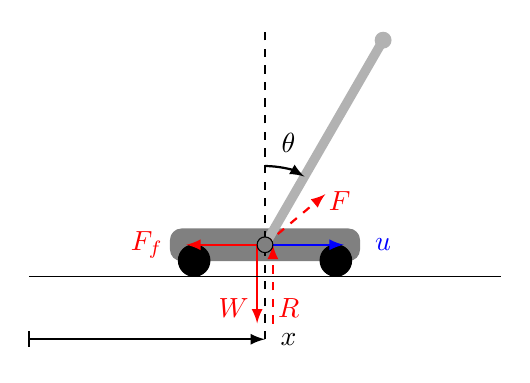
\begin{tikzpicture}[]
	
	\draw[fill=black!50, black!50, rounded corners] (-1.2,-0.2) rectangle (1.2,0.2); % body
	\draw[fill=black] (0.9,-0.2) circle (.2cm); \draw[fill=black] (-0.9,-0.2) circle (.2cm); % wheels
	\draw[black!30, line width = 1.2mm, rotate=-30] (0,0) -- (0,3); % pole
	
	\draw[-latex, blue, thick] (0, 0) -- (1,0);
	\draw[-latex, red, thick] (0, 0) -- (-1,0);
		
	\draw[dashed] (0,-1.2) -- (0,2.75);
	
	\draw[-latex, red, thick] (-0.1, 0) -- (-0.1,-1);
	\draw[-latex, red, dashed, thick] (0.1, -1) -- (0.1,0);
	\draw[red,dashed,-latex,thick,rotate=-50] (0,0) -- (0,1);
	
	\draw[rotate=90, -latex,thick] (1,0) arc (0:-30:1cm);
	\draw[fill=black!15, black!30] (1.5,2.5981) circle (1mm); 
	\draw[fill=gray] (0,0) circle (1mm);
	
	\node[] at (0.3,1.3) {$\theta$};
	
	\draw[] (-3,-0.4) -- (3,-0.4);
	
	\node[] at (0.3,-1.2) {$x$};
	\draw[thick] (-3, -1.1) -- (-3,-1.3);
	\draw[-latex,thick] (-3, -1.2) -- (0,-1.2);
	
	\node[] at (1.5,0) {\color{blue}$u$};
	\node[] at (-1.5,0) {\color{red}$F_{\te{f}}$};
	\node[] at (0.95,0.55) {\color{red}$F$};
	\node[] at (-0.4,-0.8) {\color{red}$W$};
	\node[] at (0.3,-0.8) {\color{red}$R$};

	
\end{tikzpicture}